\usepackage[paperwidth=105mm,paperheight=297mm,margin=1cm]{geometry}
\usepackage[utf8]{inputenc}
\usepackage[T1]{fontenc}
\usepackage[swedish]{babel}
\usepackage{amsmath}
\usepackage{lmodern}
\usepackage{units}
\usepackage{icomma}
\usepackage{color}
\usepackage{graphicx}
\usepackage{bbm}
\usepackage{hyperref}
\pagenumbering{gobble}
\usepackage{multicol}
\usepackage[dvipsnames]{xcolor}
\usepackage{pgfornament}

\usepackage{titlesec}
\usepackage{mathtools}
\newcommand{\orientation}{\landskap}
%% --- %%

%% Section-format %%
\setlength{\columnsep}{1.5cm}
\titleformat
{\section} % command
[display] % shape
{\bfseries\Large\itshape} % format
{} % label
{0em} % sep
{\vspace{-0.5em}\hspace{-0.05em}} % before-code
[\vspace{0em}] % after-code
\titlespacing{\section}{0em}{0em}{0.2em}
\setlength{\parindent}{0cm}
%% --- %%

%% Titelformat %%
\newcommand{\titelsida}
{
\begin{center}
\includegraphics[width=\logga]{logo.png}~\\[0.75em]
{ \Huge \titel \\[0.75em] }
{\large \datum\\\vspace{0.6em}}
{\large Sångförmän:\\ \host\\[0.5em]}
{\large Förrätt: \forratt\\\vspace{0.1em}}
{\large Huvudrätt: \huvudratt\\\vspace{0.1em}}
{\large Efterrätt: \efterratt\\\vspace{0.1em}}
\end{center}
}

\newcommand{\titelnoname}
{
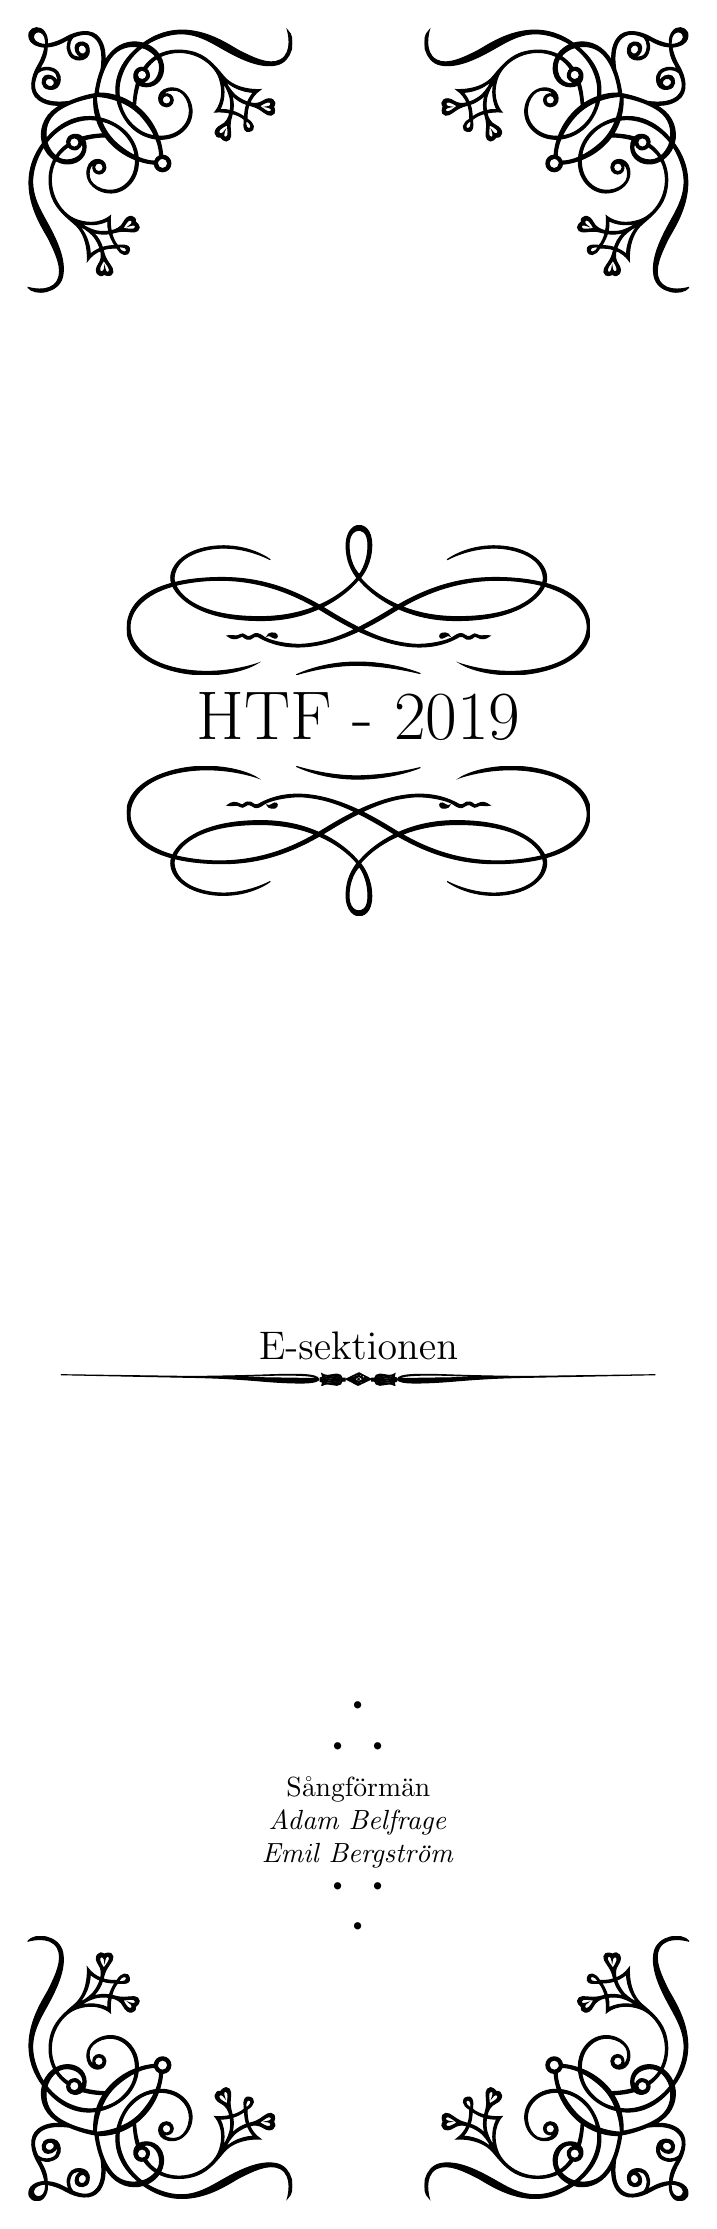
\begin{tikzpicture}[color=Black,
                        every node/.style={inner sep=0pt}]
     %\draw[help lines] (-6,-3) grid (6,3);
     \node[minimum width=84mm, minimum height=276mm](vecbox){};
%     \draw[thin, gray!20]
%          (vecbox.north west)
%       -- (vecbox.north east)
%       -- (vecbox.south east)
%       -- (vecbox.south west)
%       -- cycle;
       
\node[anchor=north west] at (vecbox.north west){%
\pgfornament[width=0.4*84mm]{61}};
\node[anchor=north east] at (vecbox.north east){%
\pgfornament[width=0.4*84mm,symmetry=v]{61}};
\node[anchor=south west] at (vecbox.south west){%
\pgfornament[width=0.4*84mm,symmetry=h]{61}};
\node[anchor=south east] at (vecbox.south east){%
\pgfornament[width=0.4*84mm,symmetry=c]{61}};
       
    \node[inner sep=6pt](text) at (0,5){
    \begin{tabular}{c}
        \Huge HTF - 2019
    \end{tabular}
    };
    \node[anchor=north] at (text.south){%
    \pgfornament[width=0.7*84mm]{75}};
    \node[anchor=south] at (text.north){%
    \pgfornament[width=0.7*84mm,symmetry=h]{75}};

    \node[inner sep=6pt](name) at (0,-3){
    \begin{tabular}{c}
        \Large E-sektionen
    \end{tabular}
    };
    \node[anchor=south] at (name.south){%
    \pgfornament[width=0.9*84mm,symmetry=h]{89}};

%    \node[inner sep=6pt](first) at (0,-1){
%    \begin{tabular}{c}
%        \Huge$\cdot$\\
%        Soppa på blomkål från Bunkeflostrand\\ med krämigt sprättägg från Stehag,\\ krispig mandelpotatis, salta frö \\och krass\\
%        \small \emph{Silverboom Chardonnay}\\
%        \Huge$\cdot$\\
%        Anka från Munka Ljungby \\med rotselleri, syrliga betor, hyvlat \\äpple och våra övervintrade kryddiga örter\\
%        \small \emph{Lindemans Bin 40 Merlot}\\
%        \Huge$\cdot$\\
%        Choklad från Valhrona, sorbet på\\ skogens bär samt krossade drömmar\\ och harsyra\\
%        \Huge$\cdot$
%    \end{tabular}
%    };
    
%    \node[inner sep=6pt](tack) at (0,-7){
%    \begin{tabular}{c}
%        Stort tack till\\
%        \emph{Ellinge Slott}\\
%        \emph{Gastrodining}\\
%        \emph{Bergkvarabuss}
%    \end{tabular}
%    };
    
    \node[inner sep=6pt](toastmaster) at (0,-9){
    \begin{tabular}{c}
        \Huge$\cdot$\\
        \Huge$\cdot$ $\cdot$\\
        Sångförmän\\
        \emph{Adam Belfrage}\\
        \emph{Emil Bergström}\\
        \Huge$\cdot$ $\cdot$\\
        \Huge$\cdot$
    \end{tabular}
    };
\end{tikzpicture}
}

\newcommand{\titelnamn}[1]
{
\begin{tikzpicture}[color=Black,
                        every node/.style={inner sep=0pt}]
     %\draw[help lines] (-6,-3) grid (6,3);
     \node[minimum width=84mm, minimum height=276mm](vecbox){};
     \draw[thin, gray!20]
          (vecbox.north west)
       -- (vecbox.north east)
       -- (vecbox.south east)
       -- (vecbox.south west)
       -- cycle;
       
\node[anchor=north west] at (vecbox.north west){%
\pgfornament[width=0.2*84mm]{61}};
\node[anchor=north east] at (vecbox.north east){%
\pgfornament[width=0.2*84mm,symmetry=v]{61}};
\node[anchor=south west] at (vecbox.south west){%
\pgfornament[width=0.2*84mm,symmetry=h]{61}};
\node[anchor=south east] at (vecbox.south east){%
\pgfornament[width=0.2*84mm,symmetry=c]{61}};
       
    \node[inner sep=6pt](text) at (0,10){
    \begin{tabular}{c}
        \Huge Vårbalen 2019
    \end{tabular}
    };
    \node[anchor=north] at (text.south){%
    \pgfornament[width=0.7*84mm]{75}};
    \node[anchor=south] at (text.north){%
    \pgfornament[width=0.7*84mm,symmetry=h]{75}};

    \node[inner sep=6pt](name) at (0,5){
    \begin{tabular}{c}
        \Large #1
    \end{tabular}
    };
    \node[anchor=south] at (name.south){%
    \pgfornament[width=0.9*84mm,symmetry=h]{89}};

    \node[inner sep=6pt](first) at (0,-1){
    \begin{tabular}{c}
        \Huge$\cdot$\\
        Soppa på blomkål från Bunkeflostrand\\ med krämigt sprättägg från Stehag,\\ krispig mandelpotatis, salta frö \\och krass\\
        \small \emph{Silverboom Chardonnay}\\
        \Huge$\cdot$\\
        Anka från Munka Ljungby \\med rotselleri, syrliga betor, hyvlat \\äpple och våra övervintrade kryddiga örter\\
        \small \emph{Lindemans Bin 40 Merlot}\\
        \Huge$\cdot$\\
        Choklad från Valhrona, sorbet på\\ skogens bär samt krossade drömmar\\ och harsyra\\
        \Huge$\cdot$
    \end{tabular}
    };
    
    \node[inner sep=6pt](tack) at (0,-7){
    \begin{tabular}{c}
        Stort tack till\\
        \emph{Ellinge Slott}\\
        \emph{Gastrodining}\\
        \emph{Bergkvarabuss}
    \end{tabular}
    };
    
    \node[inner sep=6pt](toastmaster) at (0,-11){
    \begin{tabular}{c}
        \Huge$\cdot$\\
        \Huge$\cdot$ $\cdot$\\
        Sångförmän\\
        \emph{Adam Belfrage}\\
        \emph{Emil Bergström}\\
        \Huge$\cdot$ $\cdot$\\
        \Huge$\cdot$
    \end{tabular}
    };
\end{tikzpicture}
}
%% --- %%

%% Sång %%
\newcommand{\inputsong}[1]{\input{texter/#1.tex}}
%% --- %%

% Environment for songs
\newenvironment{song}[2]{
\section{#1}
\label{#2}
}{}

% Environment for verses
\newenvironment{vers}{
\begin{flushleft}\filbreak
}{
\end{flushleft}{}
}

% Definiera melodirad
\newcommand{\mel}[1]{\begin{flushleft}\textit{\small{Mel: #1}}\end{flushleft}}
% Ta bort eventuella kommentarer i sånghäftet
\newcommand{\av}[1]{}
\newcommand{\kom}[1]{}


% Repriser sheet music
\newcommand{\repopen}
{
	\raisebox{-.4ex}{\rule{.2ex}{2.5ex}\,\rule{.1ex}{2.5ex}}
	\hspace{-0.4ex}\raisebox{.2ex}{:}
}
\newcommand{\repclose}
{
	\raisebox{.2ex}{:}\hspace{-0.4ex}
	\raisebox{-.4ex}{\rule{.1ex}{2.5ex}\,\rule{.2ex}{2.5ex}}
}

% Definiera om sidbrytningar från sjungboken till ingenting - ändra inte
\newcommand{\newp}{}